% !TEX TS-program = xelatex
% !TEX encoding = UTF-8

\documentclass[11pt,a4paper,oneside]{article}

% ── Core Packages ──────────────────────────────────────────
\usepackage[margin=2.2cm, headheight=25pt, top=2.5cm]{geometry}
\usepackage{fontspec}
\usepackage{xcolor}
\usepackage{graphicx}
\usepackage{amsmath,amssymb}
\usepackage{booktabs}
\usepackage{tabularx}
\usepackage{enumitem}
\usepackage{hyperref}
\usepackage{fancyhdr}
\usepackage{titlesec}
\usepackage{tcolorbox}
\usepackage{fontawesome5}
\usepackage{tikz}
\usepackage{pgfplots}
\usepackage{abstract}
\usepackage{setspace}
\usepackage{caption}
\usepackage{microtype}

\pgfplotsset{compat=1.18}
\usetikzlibrary{positioning,shapes.geometric,arrows.meta,calc,fit,shadows}

% ── Typography ─────────────────────────────────────────────
\setmainfont{Inter} % Requires Inter font installed, fallback to Helvetica
\setsansfont{Inter}
\setmonofont{DejaVu Sans Mono}

% ── Colors (Praxis High-Impact Palette) ────────────────────
\definecolor{praxisBlue}{HTML}{007AFF}
\definecolor{praxisPurple}{HTML}{5856D6}
\definecolor{praxisGold}{HTML}{FFD60A}
\definecolor{praxisSuccess}{HTML}{34C759}
\definecolor{praxisDark}{HTML}{050505}
\definecolor{praxisGray}{HTML}{1C1C1E}
\definecolor{praxisText}{HTML}{F2F2F7}

% Domain Colors
\definecolor{careerGreen}{HTML}{4CAF50}
\definecolor{investingTeal}{HTML}{26A69A}
\definecolor{fitnessRed}{HTML}{FF3B30}
\definecolor{academicsPink}{HTML}{AF52DE}
\definecolor{mentalBlue}{HTML}{5AC8FA}
\definecolor{philGray}{HTML}{8E8E93}
\definecolor{cultureGreen}{HTML}{32D74B}
\definecolor{romanceOrange}{HTML}{FF9F0A}
\definecolor{socialPurple}{HTML}{BF5AF2}

% ── Hyperref Setup ─────────────────────────────────────────
\hypersetup{
    colorlinks=true,
    linkcolor=praxisBlue,
    citecolor=praxisPurple,
    urlcolor=praxisBlue,
    pdftitle={PRAXIS: The Architecture of Intent},
    pdfauthor={Praxis Technologies},
    pdfsubject={Goal-Aligned Social Operating System}
}

% ── Header / Footer ────────────────────────────────────────
\pagestyle{fancy}
\fancyhf{}
\fancyhead[L]{\small\textcolor{praxisBlue}{\textbf{PRAXIS} \textbar\ Architecture of Intent}}
\fancyhead[R]{\small\textcolor{praxisGold}{CONFIDENTIAL INVESTMENT MEMO}}
\fancyfoot[C]{\small\textcolor{philGray}{\thepage}}
\renewcommand{\headrulewidth}{0.4pt}
\renewcommand{\headrule}{\hbox to\headwidth{\color{praxisPurple}\leaders\hrule height \headrulewidth\hfill}}

% ── Section Styles ─────────────────────────────────────────
\titleformat{\section}{\Large\bfseries\color{white}}{\thesection.}{0.75em}{}[\vspace{-4pt}\color{praxisPurple}\rule{\linewidth}{2pt}]
\titleformat{\subsection}{\large\bfseries\color{praxisBlue}}{\thesubsection.}{0.5em}{}

% ── Custom Boxes ───────────────────────────────────────────
\tcbuselibrary{skins,breakable}
\newtcolorbox{statbox}[1][]{
    enhanced, breakable, colback=praxisGray, colframe=praxisBlue,
    fonttitle=\bfseries\color{white}, title={#1},
    left=8pt, right=8pt, top=6pt, bottom=6pt
}

\newtcolorbox{marketbox}{
    enhanced, breakable, colback=praxisDark, colframe=praxisGold,
    coltitle=praxisGold, fonttitle=\Large\bfseries,
    title={\faRocket\quad THE OPPORTUNITY},
    coltext=white, left=12pt, right=12pt, top=10pt, bottom=10pt
}

\newtcolorbox{callout}[2][]{
    enhanced, breakable, colback=praxisGray, colframe=praxisBlue,
    fonttitle=\bfseries\color{white}, title={#2}, #1,
    left=6pt, right=6pt, top=4pt, bottom=4pt
}

% ───────────────────────────────────────────────────────────
\begin{document}

% ═══════════════════════════════════════════════════════════
%  TITLE PAGE
% ═══════════════════════════════════════════════════════════
\begin{titlepage}
\pagecolor{praxisDark}
\color{white}
\begin{center}
\vspace*{2cm}
{\fontsize{80}{90}\selectfont\textbf{\textcolor{praxisBlue}{P}RAXIS}}

\vspace{0.8cm}
{\LARGE\textbf{THE ARCHITECTURE OF INTENT}}

\vspace{1.5cm}
\textcolor{praxisPurple}{\rule{14cm}{2pt}}

\vspace{1.5cm}
{\Large\bfseries The Social Operating System for the \$6.8T Wellness Economy}

\vspace{1cm}
{\normalsize Version 2.1 \quad|\quad March 2026 \quad|\quad Built for Global Scale}

\vspace{3cm}
\begin{center}

\begin{tikzpicture}[node distance=4cm]
    \node[draw=praxisBlue, rounded corners=10pt, inner sep=15pt, align=center, fill=praxisGray] (A) {\textcolor{praxisBlue}{\Large\faBullseye}\\\textbf{Intentionality}\\\small Not Consumption};
    \node[draw=praxisPurple, rounded corners=10pt, inner sep=15pt, align=center, right of=A, fill=praxisGray] (B) {\textcolor{praxisPurple}{\Large\faLink}\\\textbf{Alignment}\\\small Not Appearance};
    \node[draw=praxisGold, rounded corners=10pt, inner sep=15pt, align=center, right of=B, fill=praxisGray] (C) {\textcolor{praxisGold}{\Large\faChartLine}\\\textbf{Validation}\\\small Not Vanity};
\end{tikzpicture}
\end{center}

\vfill
{\small\textcolor{philGray}{
    Praxis Technologies · Investor Relations · \href{mailto:ir@praxis.app}{ir@praxis.app}
}}
\end{center}
\end{titlepage}
\nopagecolor
\pagecolor{praxisDark}
\color{praxisText}

% ═══════════════════════════════════════════════════════════
%  EXECUTIVE SUMMARY
% ═══════════════════════════════════════════════════════════
\newpage
\begin{abstract}
\noindent
\textcolor{white}{\textbf{Praxis is the first Social Operating System built for Aligned Will.}} Current social graphs are broken: they optimize for attention (consumption) and shallow connections (appearance). Praxis creates a new asset class: \textbf{Verified Intentionality}. By mapping human ambition into a multi-domain semantic goal tree, Praxis uses AI-driven vector matching to pair users into high-performance accountability units. With a SaaS-FinTech hybrid model, Praxis monetizes via subscriptions, accountability escrow fees, and a future B2B marketplace. This is not a productivity app; it is the infrastructure for a more intentional species.
\end{abstract}

\tableofcontents

% ═══════════════════════════════════════════════════════════
%  1. MARKET THESIS: THE \$6.8T OPPORTUNITY
% ═══════════════════════════════════════════════════════════
\newpage
\section{Market Thesis: The \$6.8T Opportunity}

The Global Wellness Economy has reached \textbf{\$6.8 Trillion}, yet it lacks a unified social layer. People are spending billions on fitness, mental health, and personal development, but doing so in isolation.

\begin{center}
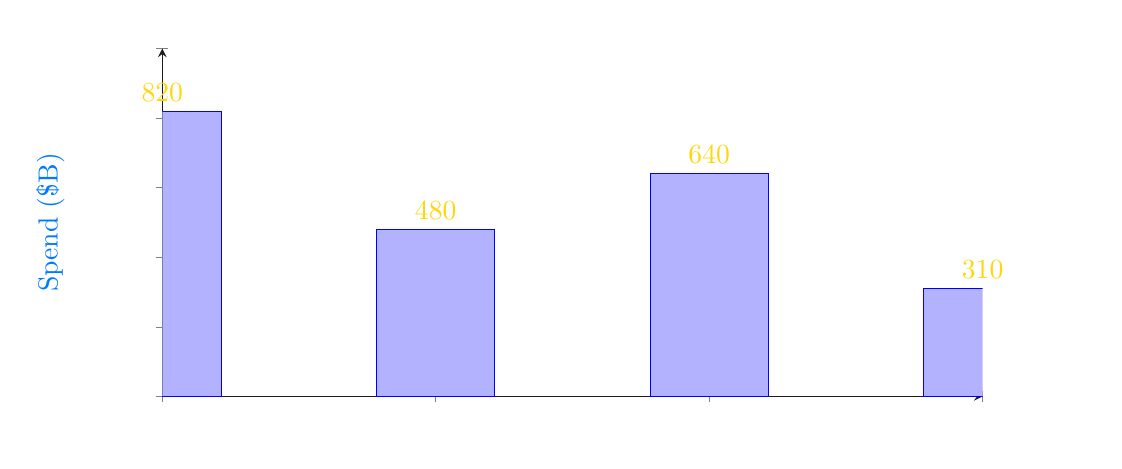
\begin{tikzpicture}
\begin{axis}[
    ybar,
    width=12cm,
    height=6cm,
    bar width=1.5cm,
    symbolic x coords={Fitness, Mental Health, Education, Personal Growth},
    xtick=data,
    axis lines=left,
    ymin=0, ymax=1000,
    ylabel={Spend (\$B)},
    axis line style={praxisGray},
    tick label style={color=white},
    label style={color=praxisBlue},
    nodes near coords,
    nodes near coords style={color=praxisGold},
    every axis plot/.append style={fill=praxisBlue!70, draw=praxisBlue}
]
\addplot coordinates {(Fitness, 820) (Mental Health, 480) (Education, 640) (Personal Growth, 310)};
\end{axis}
\end{tikzpicture}
\captionof{figure}{Annual Global Spend in Praxis-Adjacent Domains (Est. 2026)}
\end{center}

\begin{marketbox}
Praxis captures the "Serviceable Addressable Market" (SAM) of high-intent individuals. Unlike legacy platforms, Praxis is the only system that turns **Intent into a Measurable Asset**.
\end{marketbox}

% ═══════════════════════════════════════════════════════════
%  2. CORE PRODUCT: THE INTENT ENGINE
% ═══════════════════════════════════════════════════════════
\section{Core Product: The Intent Engine}

\subsection{Multi-Domain Hierarchy}
Identity is not a single point; it is a vector field across 9 life domains. 

\begin{center}
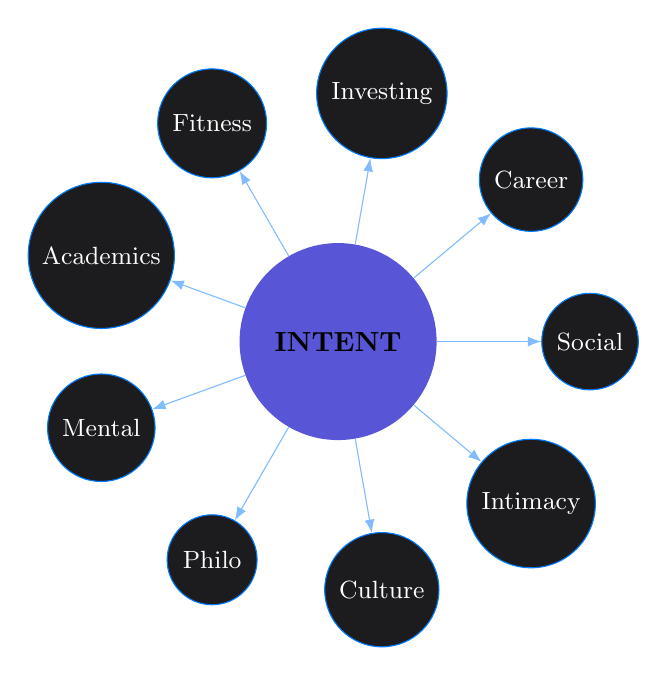
\begin{tikzpicture}[scale=0.8]
    \foreach \a [count=\i] in {Career, Investing, Fitness, Academics, Mental, Philo, Culture, Intimacy, Social} {
        \node[circle, fill=praxisGray, draw=praxisBlue, inner sep=4pt] (\i) at (\i*360/9:4) {\small\textcolor{white}{\a}};
    }
    \node[circle, fill=praxisPurple, inner sep=10pt] (Center) at (0,0) {\textbf{INTENT}};
    \foreach \i in {1,...,9} {
        \draw[arrows={-Latex}, praxisBlue!50] (Center) -- (\i);
    }
\end{tikzpicture}
\captionof{figure}{The Praxis Holistic Identity Graph}
\end{center}

\subsection{Mathematical Model of Alignment ($S_{AB}$)}
Alignment is the integral of shared semantic intent across weighted domains. The similarity score $S_{AB}$ between user $A$ and $B$ is defined as:

\begin{equation}
S_{AB} = \frac{\sum_{d \in D} w_d \cdot \cos(\vec{v}_{A,d}, \vec{v}_{B,d}) \cdot (1 - |\Delta p_d|)}{\sum_{d \in D} w_d}
\end{equation}

Where:
\begin{itemize}
    \item $w_d$: User-defined priority weight for domain $d$.
    \item $\cos(\vec{v}_{A,d}, \vec{v}_{B,d})$: Cosine similarity of 768-dim Gemini embeddings for goal descriptions.
    \item $(1 - |\Delta p_d|)$: Progress Proximity coefficient, where $p$ is progress \%.
\end{itemize}

% ═══════════════════════════════════════════════════════════
%  3. ENGAGEMENT: THE SOCIAL COMMITMENT STACK
% ═══════════════════════════════════════════════════════════
\section{Engagement: The Social Commitment Stack}

\subsection{The Reliability Score ($R$)}
The Reliability Score $R \in [0, 100]$ is the primary trust signal on the platform. It is calculated via a rolling 90-day exponential decay window:

\begin{equation}
R = \int_{t-90}^{t} (0.4C + 0.25V + 0.25M + 0.1S) \cdot e^{-\lambda(t-\tau)} d\tau
\end{equation}

\begin{itemize}
    \item \textbf{C:} Check-in Consistency.
    \item \textbf{V:} Verified Completion rate (peer-validated).
    \item \textbf{M:} Message Responsiveness.
    \item \textbf{S:} Streak Stability.
\end{itemize}

\subsection{The Network Effect Flywheel}
As the user base grows ($N$), the number of potential high-alignment matches ($M$) grows quadratically, while the "Search Latency" remains constant due to **pgvector** indexing.

\begin{center}
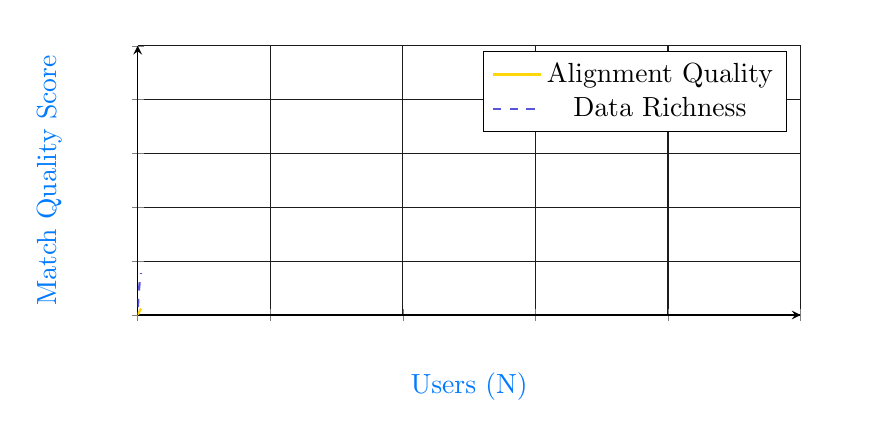
\begin{tikzpicture}
\begin{axis}[
    width=10cm, height=5cm,
    xlabel={Users (N)},
    ylabel={Match Quality Score},
    axis lines=left,
    grid=major,
    grid style={praxisGray},
    tick label style={color=white},
    label style={color=praxisBlue},
    ymin=0, ymax=100,
    xmin=0, xmax=1000
]
\addplot[thick, praxisGold, smooth] {100 * (1 - exp(-x/200))};
\addlegendentry{Alignment Quality}
\addplot[thick, praxisPurple, dashed] {20 * log10(x+1)};
\addlegendentry{Data Richness}
\end{axis}
\end{tikzpicture}
\captionof{figure}{Exponential Alignment Quality vs. User Density}
\end{center}

% ═══════════════════════════════════════════════════════════
%  4. MONETIZATION: THE HYBRID MODEL
% ═══════════════════════════════════════════════════════════
\section{Monetization: The Hybrid Model}

\subsection{5-Year Revenue Projection}
Revenue is derived from a 12\% Free-to-Paid conversion rate and a 5\% transaction fee on Accountability Staking (Escrow).

\begin{center}
\begin{tabularx}{\linewidth}{l X X X X}
\toprule
\textbf{Metric} & \textbf{Year 1} & \textbf{Year 2} & \textbf{Year 3} & \textbf{Year 5} \\
\midrule
Total Users & 50K & 250K & 1.2M & 5M \\
Paying Subscribers (12\%) & 6K & 30K & 144K & 600K \\
SaaS ARR (@ \$80 avg) & \$480K & \$2.4M & \$11.5M & \$48M \\
Staking Volume (Escrow) & \$1M & \$8M & \$45M & \$250M \\
\textbf{Praxis Fee (5\%)} & \textbf{\$50K} & \textbf{\$400K} & \textbf{\$2.25M} & \textbf{\$12.5M} \\
\midrule
\textbf{Total Gross Revenue} & \textbf{\$530K} & \textbf{\$2.8M} & \textbf{\$13.75M} & \textbf{\$60.5M} \\
\bottomrule
\end{tabularx}
\end{center}

% ═══════════════════════════════════════════════════════════
%  5. SCALABILITY: AUTOPOIETIC ZEN
% ═══════════════════════════════════════════════════════════
\section{Scalability: Autopoietic Zen}

\subsection{Axiom AI: The Balancer}
Unlike hustle-culture apps that demand 24/7 output, Praxis uses the **Axiom AI** to enforce **Sustainable Intentionality**. 

\begin{statbox}[Sustainable Growth Philosophy]
If a user is 100\% consistent in "Career" but 0\% in "Mental Health" or "Philosophy" for 14 days, the AI triggers a **Balance Intervention**. The user is nudged to take a "Zen Day" (preserving their streak) to focus on neglected domains. This increases long-term LTV (Lifetime Value) by reducing churn caused by burnout.
\end{statbox}

\subsection{B2B: The Talent Intent Marketplace}
In Year 3, Praxis will launch the **Intent Marketplace**. Companies can hire based on verified reliability and goal alignment, moving beyond the noise of traditional resumes.

% ═══════════════════════════════════════════════════════════
%  6. CONCLUSION
% ═══════════════════════════════════════════════════════════
\section{Conclusion}

Praxis is not a tool; it is a structural upgrade to the human social experience. By replacing vanity metrics with **Verified Intent**, we are building a future where your social circle is your greatest asset.

\bigskip
\begin{callout}[colback=praxisPurple!20, colframe=praxisPurple]{The Investment Bottom Line}
\centering
\Large
\textbf{Praxis is where Ambition meets Infrastructure.}\\[8pt]
\normalsize
\textit{First-to-market Intent Graph. High-Margin SaaS + FinTech Fees. Scalable AI Architecture.}
\end{callout}

\vfill
\begin{center}
\textcolor{praxisBlue}{\rule{8cm}{1.5pt}} \\
\small\textcolor{philGray}{© 2026 Praxis Technologies. Confidential Document.}
\end{center}

\end{document}
